% Uncomment this to make slides with overlays:
%\documentclass[slides]{beamer}

% Uncomment these (but comment the above \documentclass line) to make handouts:
\documentclass[handout]{beamer}

% Uncomment these to have more than one slide per page
\usepackage{pgfpages}
\pgfpagesuselayout{2 on 1}[border shrink=5mm]
\pgfpageslogicalpageoptions{1}{border code=\pgfusepath{stroke}}
\pgfpageslogicalpageoptions{2}{border code=\pgfusepath{stroke}}

\usepackage[]{graphicx, color, hyperref}

\mode<presentation>
{
	%\usetheme[secheader]{Boadilla}
	%\usecolortheme[rgb={.835, .102,.169}]{structure}  
	\usetheme[width= 0cm]{Goettingen}
	%\setbeamercovered{transparent}
}
\setbeamertemplate{navigation symbols}{}
\setbeamertemplate{footline}[frame number]

\definecolor{blue2}{rgb}{0.278,0.278,0.729} 
\newcommand{\blue}[1]{\textcolor{blue2}{#1}}
\newcommand{\white}[1]{\textcolor{white}{#1}}
\newcommand{\red}[1]{\textcolor{red}{#1}}
\newcommand{\xbar}{\overline{x}}
\newcommand{\ybar}{\overline{y}}
\newcommand{\phat}{\widehat{p}}
\newcommand{\prob}{\mbox{Pr}}
\newcommand{\E}{\mathbb{E}}
\newcommand{\Var}{\mbox{Var}}
\newcommand{\cp}{\oplus}
\newcommand{\cm}{\circleddash}


\title{Lecture 17: Paired Data and Difference of Two Means}
\author{Chapter 5.1-5.2}
\date{}


\begin{document}
%------------------------------------------------------------------------------
\begin{frame}
\titlepage
\end{frame}
%------------------------------------------------------------------------------



%------------------------------------------------------------------------------
\begin{frame}[fragile]
\frametitle{Goals for Today}

\begin{itemize}
\item Note on Practical vs Statistical Significance
\item Difference of Means
\end{itemize}

\end{frame}
%------------------------------------------------------------------------------




%------------------------------------------------------------------------------
\begin{frame}[fragile]
\frametitle{Terminology Recap (Page 192)}

\begin{itemize}
\pause\item \blue{Summary statistics} are a single number summarizing a large amount of data.\\
Ex: sample mean $\xbar=\frac{1}{n}\sum_{i=1}^{n}x_i$
\pause\item \blue{Point estimates} use observations $x_1,\ldots,x_n$ to guess at the value of an unknown parameter.  \\
Ex:  the sample mean $\xbar$ estimates the true population mean $\mu$.  
\pause\item A \blue{test statistic} is a summary statistic used in hypothesis testing or for identifying the p-value.\\
Ex:  in the Reed sleep example, we used $\xbar$.  Since $\xbar$ is approximately normal by the CLT, we use the z-score of $\xbar$ as the test statistic.  
\end{itemize}

\end{frame}
%------------------------------------------------------------------------------



%-------------------------------------------------------------------------------
\begin{frame}
\frametitle{Hypothesis Testing Procedure}\label{ht}
\begin{enumerate}
\item Construct your hypothesis testing framework:
\begin{itemize}
\item Define $H_0$, $H_A$ and if applicable a null value.
\item Set your significance level $\alpha$
\end{itemize}
\item Verify that the conditions hold
\item Compute your \blue{test statistic}
\item Compute the p-value
\begin{itemize}
\item Identify the appropriate distribution to compare the test statistic to
\item Depending on $H_A$, determine what constitutes being \blue{more extreme} and compute the p-value using the appropriate probability table.
\end{itemize}
\item If the p-value is $< \alpha$, reject $H_0$.  Otherwise do not.
\end{enumerate}

\end{frame}
%-------------------------------------------------------------------------------




%------------------------------------------------------------------------------
\begin{frame}[fragile]
\frametitle{In General:  Confidence Intervals}

All confidence intervals have form:
\begin{eqnarray*}
&& \left[\mbox{point estimate} - z^* \times SE, \ \mbox{point estimate} + z^* \times SE\right]\\
&& \mbox{point estimate } \pm \ z^* \times SE\\
&& \mbox{point estimate } \pm \mbox{ margin of error}
\end{eqnarray*}
where $z^*$ determines the confidence level.

\pause\vspace{0.25cm}

The point estimate and $SE$ will change depending on the context.  

\end{frame}
%------------------------------------------------------------------------------



%-------------------------------------------------------------------------------
\begin{frame}
\frametitle{The 8 Types of Questions}

Here are the 8 broad types of questions we can answer with statistical methods (confidence intervals and hypothesis tests) in this class: 

\vspace{0.25cm}

\begin{enumerate}
\pause\item What is the mean value $\mu$?
\pause\item Are the means of two groups $\mu_1$ and $\mu_2$ equal or not?
\pause\item What is the mean paired difference $\mu_{diff}$?
\pause\item What is the proportion $p$ of ``successes''?
\pause\item Are the proportions of ``successes'' of two groups $p_1$ and $p_2$ equal or not?
\pause\item Are the means $\mu_1, \ldots, \mu_k$ of $k$ groups \blue{all} equal or not?
\pause\item Are we observing what we were expecting?
\pause\item Are two categorical variables independent?
\end{enumerate}

\end{frame}
%-------------------------------------------------------------------------------







%total <- hist(run10Samp$time)
%F <- hist(run10Samp$time[run10Samp$gender=="F"])
%M <- hist(run10Samp$time[run10Samp$gender=="M"])
%
%mean.m <- mean(run10Samp$time[run10Samp$gender=="M"])
%mean.f <- mean(run10Samp$time[run10Samp$gender=="F"])
%
%pdf("./7.3 Paired Data + Diff of Two Mean/race.pdf", width=6, height=6)
%hist(run10Samp$time[run10Samp$gender=="M"], breaks=total$breaks, col='cyan',
%     border='cyan', xlab="Race Time (in minutes)", main="Cherry Blossom Run Times", 
%     ylim=c(0,max(F$counts, M$counts)))
%hist(run10Samp$time[run10Samp$gender=="F"],add=T)
%legend("topright", 
%       legend=c("men", "women"), 
%       fill=c("cyan", "white"),
%       bty='n')
%dev.off()
%------------------------------------------------------------------------------
\begin{frame}[fragile]
\frametitle{Are the means of two groups $\mu_1$ and $\mu_2$ equal or not?}

Example from Chapter 5.2:  Did men (n=45) run faster than women (n=55)?
\begin{center}
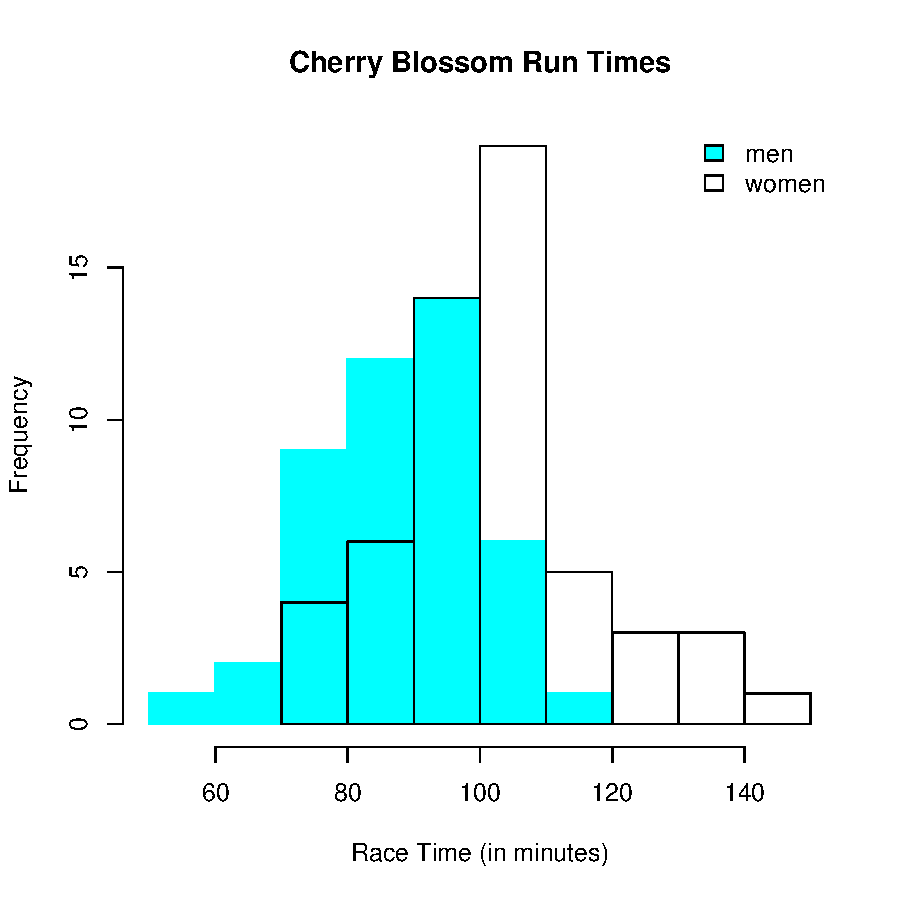
\includegraphics[width=0.6\textwidth]{figure/race.pdf}
\end{center}

\end{frame}
%------------------------------------------------------------------------------


%------------------------------------------------------------------------------
\begin{frame}[fragile]
\frametitle{Difference in Means}
We are interested in the difference of two population means $\mu_w - \mu_m$ where
\pause\begin{itemize}
\item $\mu_w$ is the mean time for women
\item $\mu_m$ is the mean time for men
\end{itemize}

\pause\vspace{0.5cm}
The data:
\begin{center}
  \begin{tabular}{c|rr}
     & men & women \\ 
\hline
    $\overline{x}$ & 87.65 & 102.13 \\ 
    $s$ & 12.5 & 15.2 \\ 
    $n$ & 45 & 55 \\ 
\end{tabular}
\end{center}

\end{frame}
%------------------------------------------------------------------------------


%------------------------------------------------------------------------------
\begin{frame}[fragile]
\frametitle{Difference of Means}
We now recreate all the elements of Chapter 4 using this new \blue{population parameter}  $\mu_w - \mu_m$:

\vspace{0.25cm}

\begin{enumerate}
\pause\item Determine a point estimate of $\mu_w - \mu_m$.
\pause\item Show the normality of the sampling distribution:  mean and SE
\pause\item Build a confidence interval
\pause\item Conduct hypothesis tests
\end{enumerate}

\vspace{0.25cm}

\pause First, the \blue{point estimate} for $\mu_w - \mu_m$ is the \blue{sample difference of means}
\[\xbar_w - \xbar_m = 102.13-87.65=14.48\]



\end{frame}
%------------------------------------------------------------------------------


%------------------------------------------------------------------------------
\begin{frame}[fragile]
\frametitle{Normality of Sampling Distribution}
If the sample means $\xbar_1$ and $\xbar_2$ 
\begin{itemize}
\pause\item each meet the criteria for having nearly normal sampling distributions
\pause\item also \blue{the observations from the two samples are independent}
\end{itemize}
\pause then the difference in sample means $\xbar_1 - \xbar_2$ will also have a nearly normal sampling distribution...

\end{frame}
%------------------------------------------------------------------------------


%------------------------------------------------------------------------------
\begin{frame}[fragile]
\frametitle{Normality of Sampling Distribution}
with 
\begin{itemize}
\pause\item mean $\mu_1-\mu_2$
\pause\item estimated standard error
\[
SE_{\xbar_1 - \xbar_2} = \sqrt{\frac{s_1^2}{n_1} + \frac{s_2^2}{n_2}}
\]
\end{itemize}
\pause Note the different $s^2$'s and sample sizes.  
\end{frame}
%------------------------------------------------------------------------------



%------------------------------------------------------------------------------
\begin{frame}[fragile]
\frametitle{Normality of Sampling Distribution}

We verify the conditions:
\begin{itemize}
\pause\item Because each sample consists of less than 10\% of their respective populations (men: 45 of 7192 and women: 55 of 9732).
\pause\item The observations for both groups don't look too skewed.
\pause\item Each sample has at least 30 observations (rule of thumb).
\pause\item The samples are independent (not paired or linked in any way).
\end{itemize}


\pause\vspace{0.25cm}
the sampling distribution is Normal with mean=$\mu_w - \mu_m$ and
\[
SE_{\xbar_w - \xbar_m} = \sqrt{\frac{15.2^2}{55} + \frac{12.5^2}{45}} = 2.77
\]

\end{frame}
%------------------------------------------------------------------------------




%------------------------------------------------------------------------------
\begin{frame}[fragile]
\frametitle{Confidence Interval}

A 95\% confidence interval for $\mu_1 - \mu_2$ is
\begin{eqnarray*}
(\mbox{point estimate for } \mu_1 - \mu_2) \pm 1.96 \times SE\\
\pause(\xbar_1 - \xbar_2) \pm 1.96 \times SE_{\xbar_1 - \xbar_2}
\end{eqnarray*}

\pause So for the Cherry Blossom Run data, a 95\% CI for $\mu_w - \mu_m$ is:
\begin{eqnarray*}
14.48 \pm 1.96 \times 2.77 =  [9.05, 19.91]
\end{eqnarray*}

\end{frame}
%------------------------------------------------------------------------------





%------------------------------------------------------------------------------
\begin{frame}[fragile]
\frametitle{Next Time}

\begin{itemize}
\item Hypothesis test for differences in means
\item Paired differences
\item One sample t-test
\end{itemize}


\end{frame}
%------------------------------------------------------------------------------





\end{document}

















\end{document}










